In validation phase an approach that uses VTM technique and the associated tool - Projection Explorer (PEx) - were applied to support the inclusion and exclusion decisions~\cite{Malheiros:2007}. %PEx adopts a two-dimensional visual representation, known as document map, where each document is mapped to a graphical element on the plane, usually a circle (point), with points relative positions reflecting similarity relationships between the contents of the documents they represent. Thereby, on the layout, similar documents are put close to one another, while dissimilar ones are supposed to be positioned far apart.

\begin{figure}[!h]
\centering
  % Requires \usepackage{graphicx}
 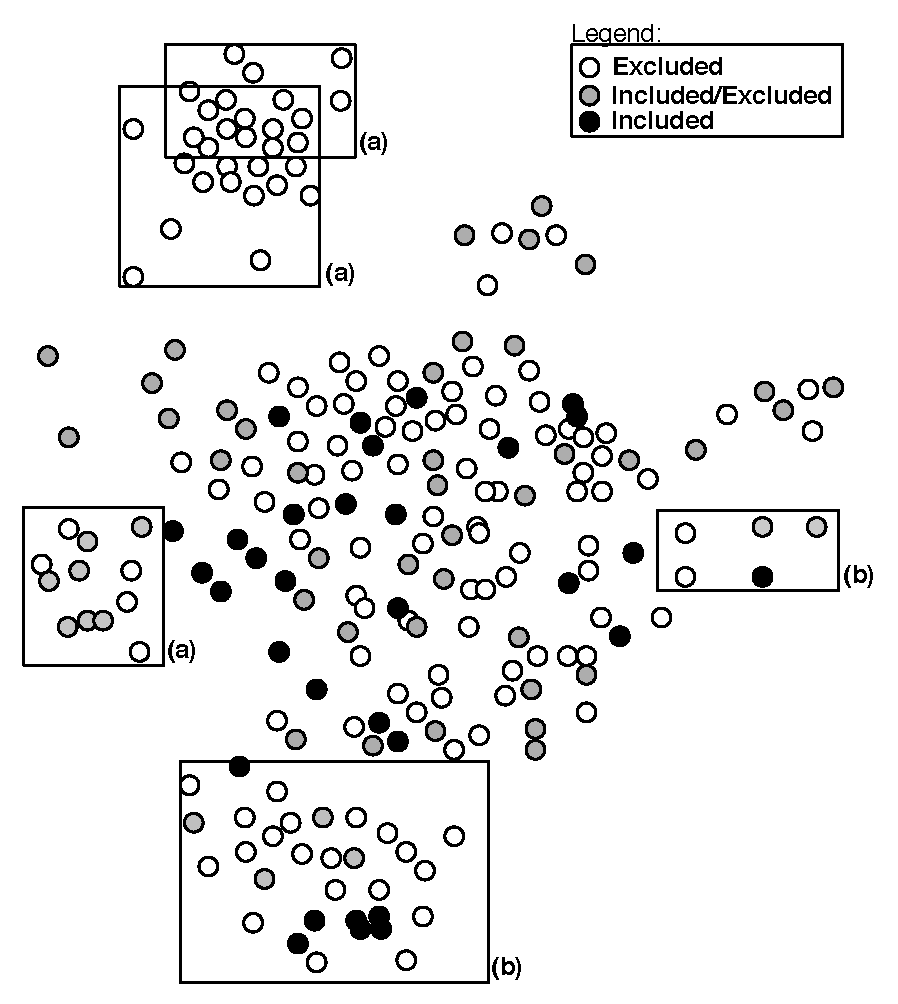
\includegraphics[scale=0.40]{figuras/validation2}
\caption{Document map colored with the history of the inclusions and exclusions of the studies.}
\label{fig:validation}
\end{figure} 

Figure~\ref{fig:validation} presents a document map generated using PEx. This map is composed of 802 primary studies analysed in this review, highlighting them using different shades of gray to differentiate in which of the stages a study was removed from the review. White points are studies excluded in first stage, gray points are the studies excluded in second stage and the black points are the included. The exploration of a document map is conducted in two steps: (\textit{i}) firstly, a clustering algorithm is applied to the document map, creating groups of highly related documents; (\textit{ii}) secondly, the resulting clusters are analysed in terms of:~\textbf{Pure Clusters} - all documents belonging to a cluster have the same classification (all included or excluded, regardless of exclusion stage). Normally, in this case do not need to be reviewed; and~\textbf{Mixed Clusters} - which represent documents with different classification on the same cluster. These cases are hints to the reviewer, and the estuaries grouped should be reviewed following the traditional method. To facility the visualisation, in Figure~\ref{fig:validation} just five clusters generated by PEx are depicted. Examples of pure clusters (all excluded) are identified in Figure~\ref{fig:validation} using label ``(a)'' and therefore do not needed to be reviewed. Mixed clusters (clusters containing black (included) and white or gray (excluded) studies) are identified using label ``(b)'' and they were reviewed by the authors of this paper. At the end, we kept the initial classifications conducted manually, but this technique contributed to a review of studies that could have been wrongly excluded or included previously.  

